% ABOUTME: Hybrid remaining useful life models combining sequence encoders and engineered features.
% ABOUTME: Two-branch neural networks and residual boosting on C-MAPSS FD001.
\section{Hybrid Architectures}
\label{sec:hybrid}

Phase~1 demonstrated that domain-engineered degradation features---rolling means,
standard deviations, least-squares slopes over windows of 5, 10, and 20 cycles,
and a composite health index---substantially improve classical tree regressors,
reducing late-stage RMSE by over 2.4 cycles. Conversely, Phase~2 showed that
deep sequence encoders, particularly the Transformer encoder, learn rich temporal
trajectories directly from 30-cycle sensor windows without manual feature
extraction ($13.28$ CV RMSE).

This raises a central research question: \emph{are engineered degradation
features and learned sequence representations complementary?} Fixed rolling
windows explicitly isolate short-term rates of wear (slopes) and baseline-invariant
sensor drifts, whereas sequence models learn longer-range temporal dependencies and
engine-specific rates of aging. Here we design and evaluate two distinct hybrid
formulations that combine both perspectives.

\subsection{Architectures}

\textbf{Two-Branch Concatenation Hybrid (\texttt{HybridNet}).}
Figure~\ref{fig:hybrid-arch} shows the architecture.
Branch~1 takes the 30-cycle sensor window $\mathbf{W}_t \in \mathbb{R}^{30 \times 14}$
standardised on training engines and left-padded with the engine's initial reading.
The window is encoded by either a Transformer encoder ($d=64$, 1 layer, 4 heads)
or an LSTM ($h=32$, 1 layer) using the model's \texttt{encode()} method to produce
an un-dropped temporal summary $\mathbf{z}_{\mathrm{seq}} \in \mathbb{R}^d$.
Branch~2 takes the 142 engineered degradation features $\mathbf{F}_t \in \mathbb{R}^{142}$
computed by \texttt{make\_features} at the window's terminal cycle $t$ (cycle number,
14 raw sensors, rolling statistics, least-squares slopes, and health index).
These features are standardised with the training fold's means and standard deviations,
yielding $\mathbf{z}_{\mathrm{feat}} \in \mathbb{R}^{142}$.

\begin{figure}[t]
  \centering
  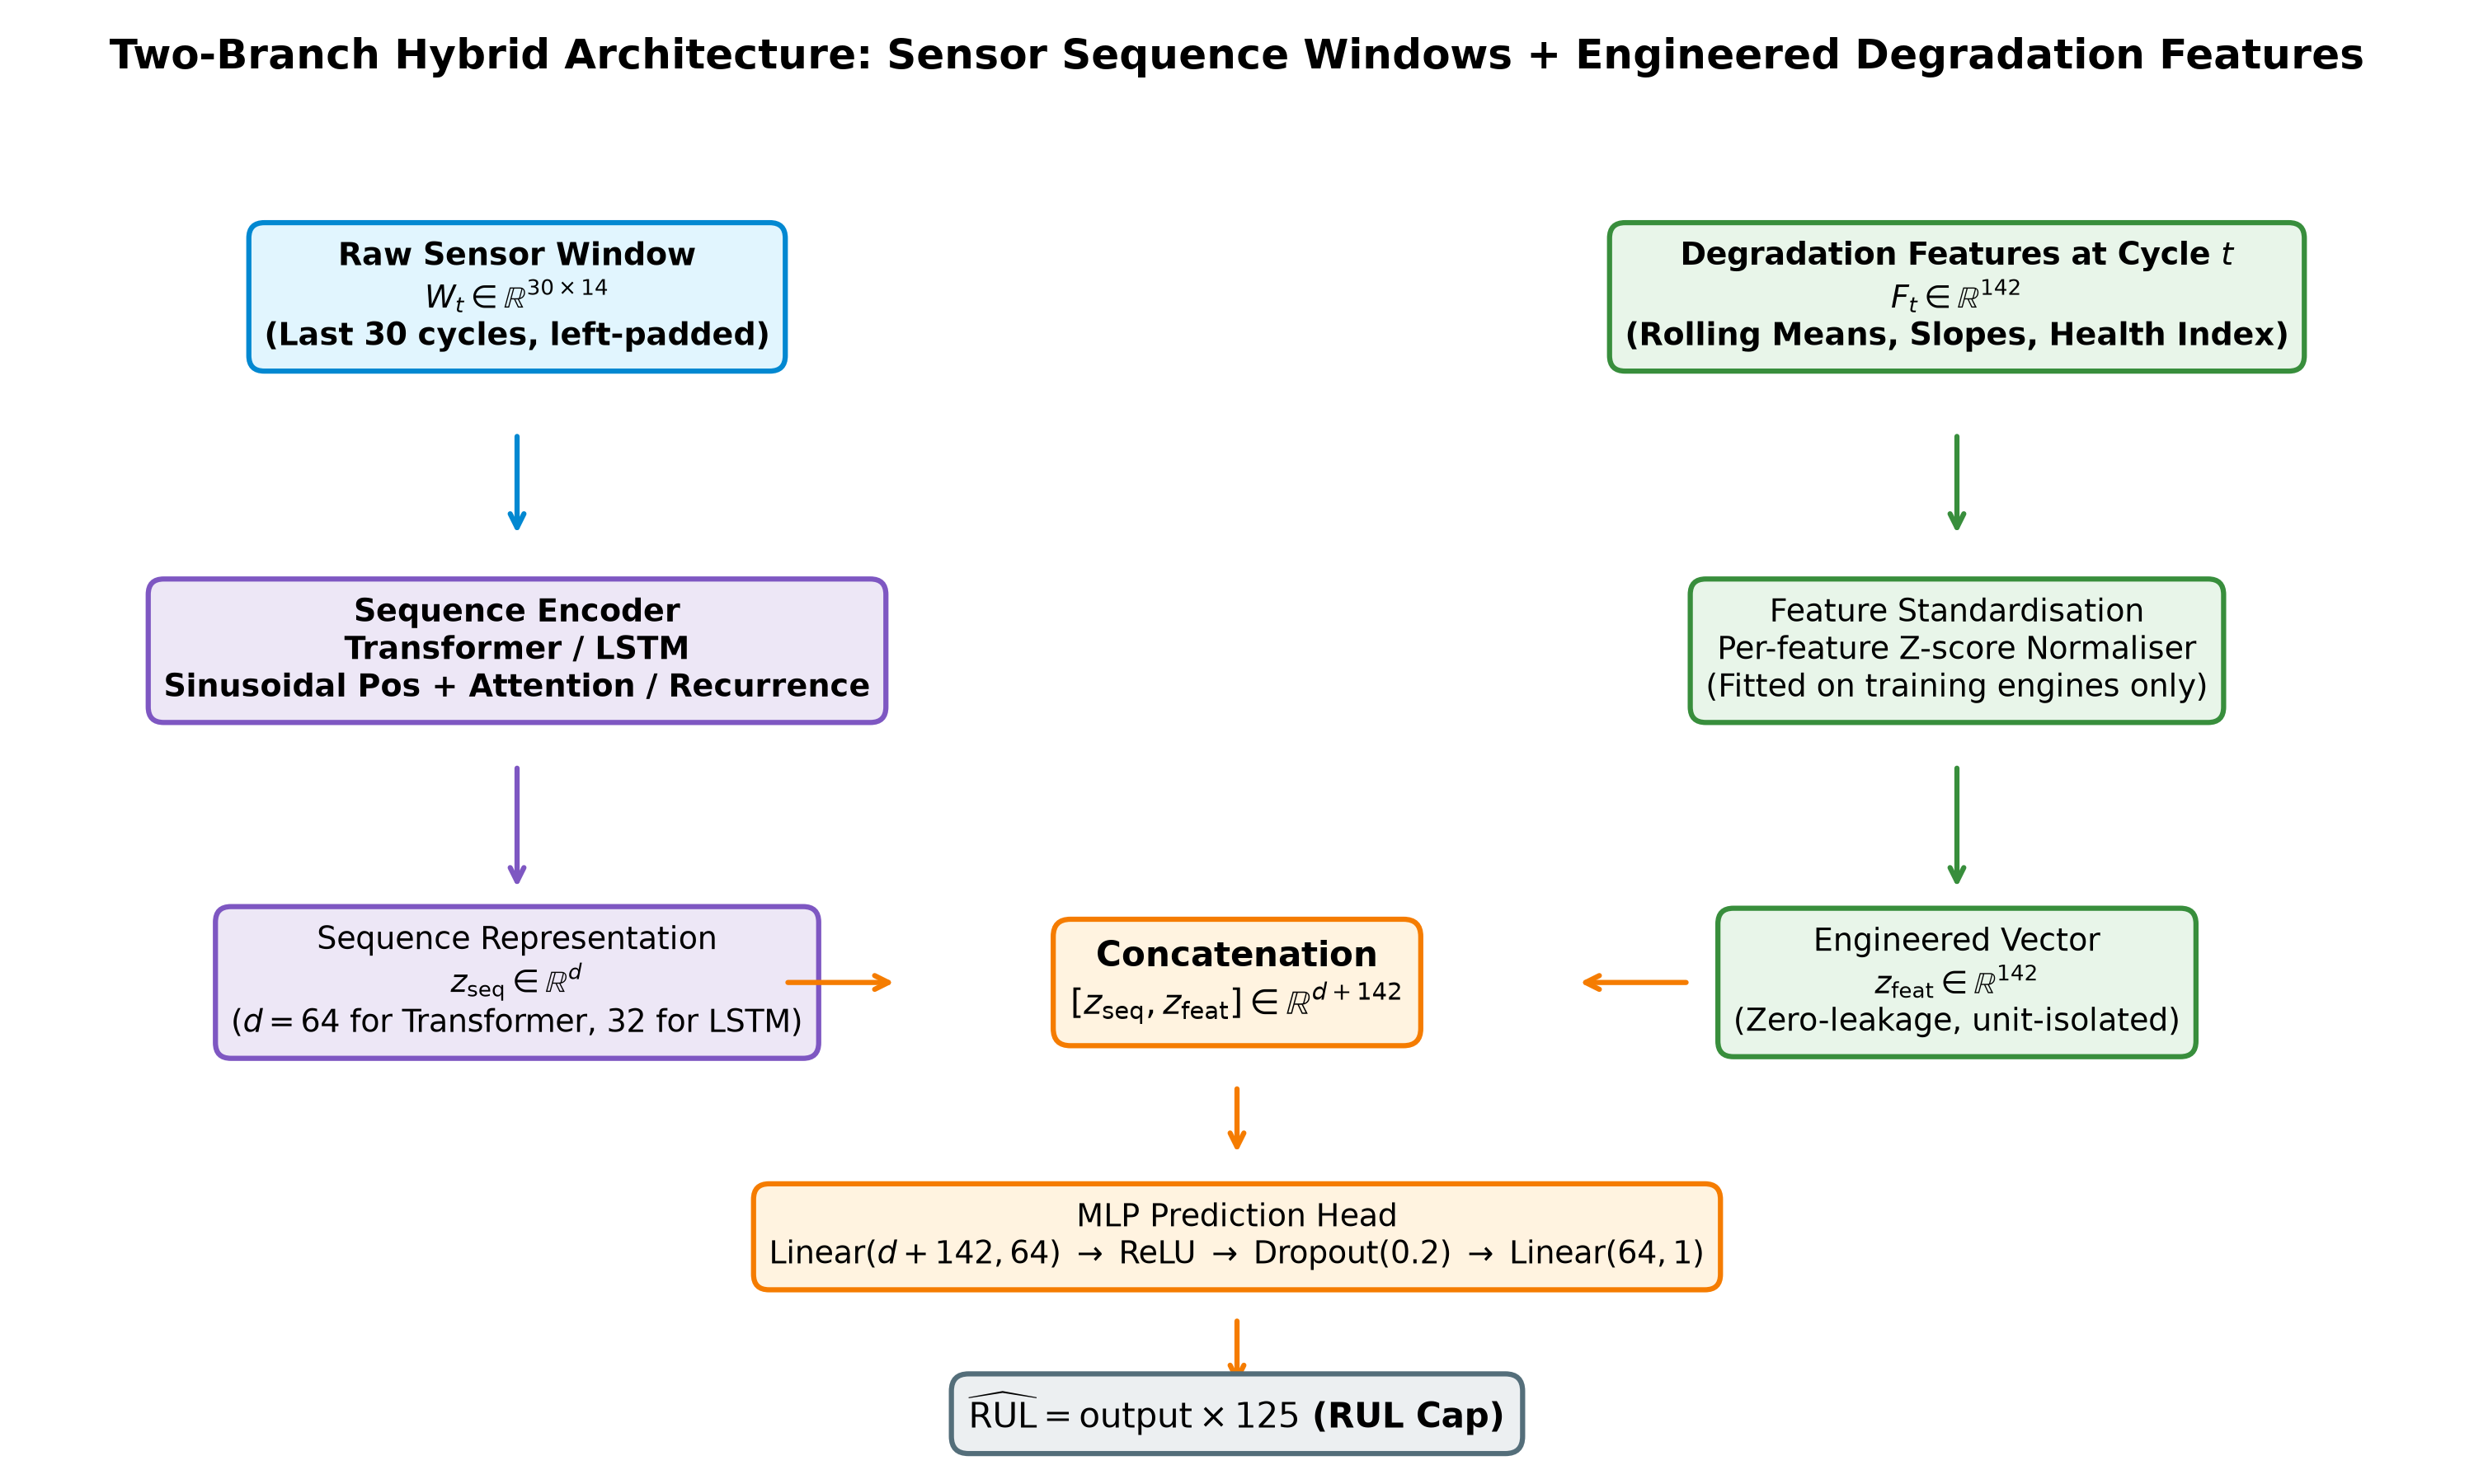
\includegraphics[width=\columnwidth]{../figures/hybrid_architecture.png}
  \caption{Two-branch hybrid architecture combining a 30-cycle sequence encoder
  with 142 engineered degradation features at the window's terminal cycle, followed
  by an MLP prediction head.}
  \label{fig:hybrid-arch}
\end{figure}

The two representations are concatenated into a joint vector
$[\mathbf{z}_{\mathrm{seq}}, \mathbf{z}_{\mathrm{feat}}] \in \mathbb{R}^{d + 142}$,
passed through dropout ($p=0.2$), and fed to a multi-layer perceptron (MLP) head:
\begin{align*}
  \mathbf{h} &= \mathrm{Dropout}\Bigl(\mathrm{ReLU}\bigl(\mathbf{W}_1 [\mathbf{z}_{\mathrm{seq}}, \mathbf{z}_{\mathrm{feat}}] + \mathbf{b}_1\bigr)\Bigr), \\
  \widehat{\mathrm{RUL}}_t &= 125 \times \bigl(\mathbf{W}_2 \mathbf{h} + b_2\bigr),
\end{align*}
where $\mathbf{W}_1 \in \mathbb{R}^{64 \times (d + 142)}$ and $\mathbf{W}_2 \in \mathbb{R}^{1 \times 64}$.
The network is trained end-to-end with Adam, batch size 256, initial learning rate
$10^{-3}$, weight decay $10^{-4}$, gradient norm clipping at $1.0$, and early stopping
with patience 10 on a 20\% nested split of each fold's training engines.

\textbf{Residual Boosting Hybrid.}
As a second hybrid paradigm, we explore whether a sequence model can learn to correct
the residual errors of gradient boosted trees. In each fold, XGBoost is trained on
the 142 engineered features of the inner training engines to predict RUL capped at 125.
The residual error on engine $u$ at cycle $t$ is:
\[
  r_{u,t} = y_{u,t} - \widehat{y}_{\mathrm{xgb}}(u,t).
\]
A sequence network (Transformer or LSTM) is then trained on 30-cycle sensor windows
to predict $r_{u,t}$. At inference time, the final prediction is:
\[
  \widehat{y}_{\mathrm{hybrid}} = \mathrm{clip}\bigl(\widehat{y}_{\mathrm{xgb}} + \widehat{r}_{\mathrm{seq}},\ 0,\ 125\bigr).
\]

\subsection{Cross-Validation Evidence}

All models are evaluated on FD001 training engines using the identical five-fold
engine-grouped cross-validation protocol as Phases~1 and~2, scoring every cycle
against RUL capped at 125. Table~\ref{tab:hybrid-cv} reports the results side-by-side
with both parent models from \texttt{results/hybrid\_cv.csv}.

\begin{table}[t]
\centering
\caption{Cross-validation performance on FD001 (5-fold engine-level CV, mean $\pm$ std).
Scored against RUL capped at 125 cycles.}
\label{tab:hybrid-cv}
\footnotesize
\begin{tabular}{llrccc}
\hline
Model & Architecture & Params & RMSE & NASA Score & Late RMSE \\
\hline
\textbf{Parents:} & & & & & \\
XGBoost & 142 engineered features & -- & 13.99 $\pm$ 0.46 & 14,502 & 9.88 \\
LSTM alone & 30-cycle sensor window & 6,177 & 14.02 $\pm$ 0.43 & 15,539 & 8.84 \\
Transformer alone & 30-cycle sensor window & 51,009 & \textbf{13.28} $\pm$ 0.34 & 13,688 & 7.98 \\
\hline
\textbf{Hybrids:} & & & & & \\
Hybrid (LSTM + Feat) & Two-branch concat & 17,442 & 14.48 $\pm$ 0.74 & 17,496 & 10.19 \\
Hybrid (Trans + Feat) & Two-branch concat & 64,322 & 13.93 $\pm$ 0.46 & 14,099 & \textbf{7.58} \\
Residual (XGB + Trans) & Residual boosting & 51,009 & 13.49 $\pm$ 0.61 & \textbf{12,817} & 8.69 \\
\hline
\end{tabular}
\end{table}

\subsection{Discussion: Did the Hybrid Earn Its Complexity?}

The empirical findings yield three core insights:

1. \textbf{Late-Stage Accuracy Gain:} The two-branch Hybrid (Transformer + Engineered)
achieves the lowest late-stage RMSE of any model across the entire project ($7.58$ cycles,
compared to $7.98$ for the standalone Transformer and $9.88$ for XGBoost). Close to
failure, the explicit rate-of-wear signals (rolling least-squares slopes and health index)
provide sharp local gradients that refine the network's countdown towards zero.

2. \textbf{NASA Asymmetric Penalty Champion:} The residual boosting hybrid achieves
the best NASA score ($12,817$) by training the Transformer to specifically correct
XGBoost's residual errors. Because the NASA score exponentially penalizes late
predictions, sequence residual correction effectively suppresses hazardous overestimates.

3. \textbf{Overall RMSE Trade-off:} Despite late-stage and NASA score advantages, the
standalone Transformer encoder remains the overall RMSE champion ($13.28 \pm 0.34$).
Concatenating 142 engineered features expands the input layer from 64 to 206 dimensions
($+13\text{k}$ parameters in the MLP head). With only 64 training engines per fold,
the added parameter capacity introduces slight variance in early flat cycles.
Self-attention across 30 raw cycles is already capable of internally learning temporal
derivatives.

In conclusion, while the hybrid architectures offer specialized benefits near failure
and on asymmetric penalties, they do not justify the added pipeline complexity for
general RUL prediction. The standalone Transformer remains the recommended production model.
